% --------------------------------------------------
% Method
% --------------------------------------------------
\chapter{The Solution Approach} \label{solapp}
% Here you should identify and evaluate the solution options against your problem statement / technical specification and make a reasoned choice of your chosen solution approach. Why did you do what you did? Conclude with a succinct definition of your solution approach and criteria by which the solution would be accepted as adequately verified. It is very likely that you will add further reference material in this section.

\section{Solutions for Environment Virtualisation} \label{subapp-virt}
In order to provide users with the most 'local' experience as possible on a remote platform it is key to analyse various technologies and techniques that are currently in widespread use in the industry. As discussed during Chapter \ref{lit} there is an consensus in the industry that containers are the better solution for PaaS type software of which this project would fall into the category of.

There are many different container solutions available currently, many have similar roots such as a backbone of using LXC but they build on top of those foundations in varying ways. Some of these ways are documented in the paper which was discussed in Section \ref{lit-containers} \cite{contsvsvirt}. This paper performed a comparison of the various different container technologies and stacked them against each other on key implementation features such as performance and security.

The decision to not research Virtual Machines as a potential solution for the system is due to the project not requiring the utility of a hypervisor. As almost all developer tools are freely available through most Linux distributions. This means that there are few to no downsides of using a container based solution versus a fully blown Virtual Machine set up and many benefits.

\subsection{Container Providers} 

A big limitation of OpenVZ is that it can't run on the standard Linux kernel so it is not a very viable solution for this project as the aim to to deploy the system and requiring a modified kernel will add complexity.

\subsection{Virtualisation Conclusion}

For the system, Docker seems to be the clear choice as it provides good tooling with its daemon. A strong foundation on top of LXC, and it doesn't require additional modification before it can be used on a computer/server which is preferable to avoid for this project.

\section{Chosen Solution for Real-Time Communication} \label{solapp-rtc}

Based off the research performed in Section \ref{lit-rtc} it would seem as though WebSockets fit the requirement of the project in order to ensure rapid communication between the client and their virtual development environment.

By using WebSockets it will be possible to have incredibly low latency bidirectional messages sent from the client to the server which can give the server instructions on what to do with the container that the client is allocated. The ability to send structured data chunks in string form makes it perfect for sending code and returning the output that is executed by the container.

WebSockets are available through the native Web APIs and so no 3rd party dependency is required to interact with them on the client side.

On the server side there are a few ways to implement a WebSocket endpoint but as Node.js and Express are already being used for the REST api it using a 3rd party dependency such as \texttt{express-ws} makes the most sense.

\section{Requirements for Frontend} \label{solapp-frontend}

In order to create an experience that emulates a local installation of tooling and a text editor it is necessary to make sure that a tooling solution is chosen for this project that can meet these needs. The key requirements for the user facing side of this project are:

\begin{enumerate}
  \item Text Editor with essential features that users expect in a standard developer environment
  \item A terminal emulator that can display output of code to users and allow input where it is appropriate
\end{enumerate}

Without these two features there is no way to adequately provide users with an environment that can be anywhere near the level of quality that they would expect from a local installation of tools.

\subsection{Text Editor}

A text editor is a vital part of a developers tool-chain and a few solutions exist on that can be rendered in the web browser. The reason a simple text input cant be used is that a text editor performs actions such as automatic indentation which, while could be recreated, is very specific to languages where for some indentation doesn't matter and for some it is how the language detects what code belongs to what block or function.

With this in mind it is helpful to establish a list of features that are a key requirement for any text editor.

\begin{itemize}
  \item Automatic indentation
  \item Syntax colouring
  \item Control + F compatibility for Find
  \item Bracket matching
  \item Copy-Paste compatibility
\end{itemize}

With these features in mind it is now worth investigating the available resources to see which one satisfies the features best and if any bonus features cna be found.

\subsubsection{Ace - \textit{https://ace.c9.io/}}

Ace is a code editor which is used by Amazon in order to provided their cloud based IDE 'Cloud9' it offers all the features that are listed above and notably includes support for themes, multiple cursors and bracket highlighting.

It's worth noting that Ace is first and foremost a code editor for online use and isn't available for users to install locally.

\subsubsection{CodeMirror - \textit{https://codemirror.net/}}

CodeMirror is another code editor that is exclusive to the browser, it is the code editor that both Firefox, Chrome and Safari use inside their dev tools. It offers all the same features as Ace, however it has a more modern design which more accurately resembles a locally installed text editor.

CodeMirror claims to have experimental support for mobile browsers however it isn't an experience that is good enough to consider as a bonus feature for the editor.

\subsubsection{Monaco - \textit{https://microsoft.github.io/monaco-editor/index.html}}

The Monaco text editor is made by Microsoft and used in their very popular code editor 'VSCode'. VSCode is one of the most popular text editors at the moment for a variety of different developer communities such as web developers and people starting out with a new language that don't want to have to deal with a fully blown IDE.

Feature-wise it offers all the features that are offered by CodeMirror and Ace but also comes built in with auto complete support for TypeScript, JavaScript, HTML and CSS. Through language servers as well, any language can gain support for auto complete for the standard language syntax. It also comes with a 'diff-editor' mode which can be used to gently introduce users to the idea of version control.

Monaco does not have as many themes available as the alternatives but the features that it does offer outweighs the value that alternate themes provides.

\subsubsection{Decision on Text Editor}

Based on the details above it makes a huge amount of sense to use the \textbf{Monaco Editor}, being provided by Microsoft is a significant benefit and the fact that it powers one of the most popular code editors that is being used in the industry means that it will provide as close an experience to a local coding environment as any of the other options.

Giving users experience with this tool will mean the transition to local development tools will be less abrasive as they already know the features that are available in these industry tools. The ability to provide auto complete for some languages is a huge benefit as well as new developers can be sure that the syntax they write is correct.

\subsection{Xterm.js Terminal Emulator - https://xtermjs.org/}

For online emulation of a terminal/command line the most popular solution is \textbf{Xterm.js} which has widespread adoption across many developer tools that require emulation of a terminal. It is used with VSCode in order to give users access to their local shell. It is highly performance focused in order to provide low to no latency between keystrokes and when they render on the screen. It also provides an array of addons that mean the terminal can be connected to a WebSocket stream so the online terminal can be connected to a real terminal on a machine. This is a key feature of a local development environment and therefore Xterm.js is ideal for this project.

\section{Solution for Building the Interface} \label{solapp-tools}

With the solutions established above it is now appropriate to evaluate the options when it comes to how to build the whole user facing side of the system.

As the developer has the most experience building websites using the \texttt{React} library (https://reactjs.org/) to help with creating reactive, data driven, single page web applications, that is the overarching technology that will be used to build the solution.

Within the React ecosystem however, there is a number of options about how to manage certain essential features such as page routing and how to style components in a way that fits into the React methodology.

\subsection{React Framework Options}

In order to get started with React the recommended way is to use a package called \texttt{create-react-app} however a limitation of this method is that it is not configurable to the extent that is required by the Monaco code editor if syntax colouring is considered a key feature, which it is.

It is necessary then to evaluate some other options for getting started with a React application that allows for the configuration options that means syntax colouring works.

The popular options in the community are: ejecting a CRA project, Next.js or Razzle.

\subsubsection{Eject Create-React-App}
Ejecting a CRA provides the developer with full access to all the configuration options that are previously abstracted away. It also installs a lot of dependencies that need to be maintained correctly and the configurable options are overwhelming when all that's required is a few lines added to a config file. This solution is undesirable.

\subsubsection{Next.js - https://nextjs.org/}
Next.js advertises itself as a React 'framework' as it provides many additional features out of the box versus traditional CRA projects. It offers functionality for:

\begin{itemize}
  \item Routing via the File System
  \item Code Splitting
  \item Server Side Rendering
  \item High Level Configuration
\end{itemize}

With these features, fewer external dependencies are required and the configuration which is needed to get syntax colourisation working is available.

\subsubsection{Razzle - https://github.com/jaredpalmer/razzle}

Razzle attempts to find a middle ground between the opinionated decisions made by Next.js and the overwhelming amount of configuration that is required after ejecting an app created by CRA. It is also agnostic to the technology that you use it with so it can be used with several other different frontend libraries such as \textit{Vue.js}.

Due to the less opinionated nature of the project the only real benefit provided by it is the server side rendering and configuration options that is also provided by Next.js.

Despite similar configuration extensibility as Next.js trying to enable syntax colouring for the Monaco editor didn't work.

\subsection{Conclusion on Frontend Framework}

As syntax colouring has been described as a key feature there isn't much of a choice beyond choosing to use either Next.js or the Ejected CRA. As Next.js has a number of other benefits however, this makes it the most attractive and powerful option for building the frontend.

\section{Design Prototypes} \label{solapp-design}

Trying to build a system that provides users with an environment where they feel as though there's not a high barrier to entry involves a design process which has to ensure that things are arranged in as friendly a way as possible.

Some sketches were done in order to try to narrow down what kind of design language should be used to give the users a sense of friendless versus the more stark, professional look that some developer focused websites aim for \texttt{StackOverflow dot com}. Based on these general requirements the following low fidelity prototypes were created presenting different ways that information could be displayed for users.

\begin{figure}[!htb]
  \minipage{0.32\textwidth}
  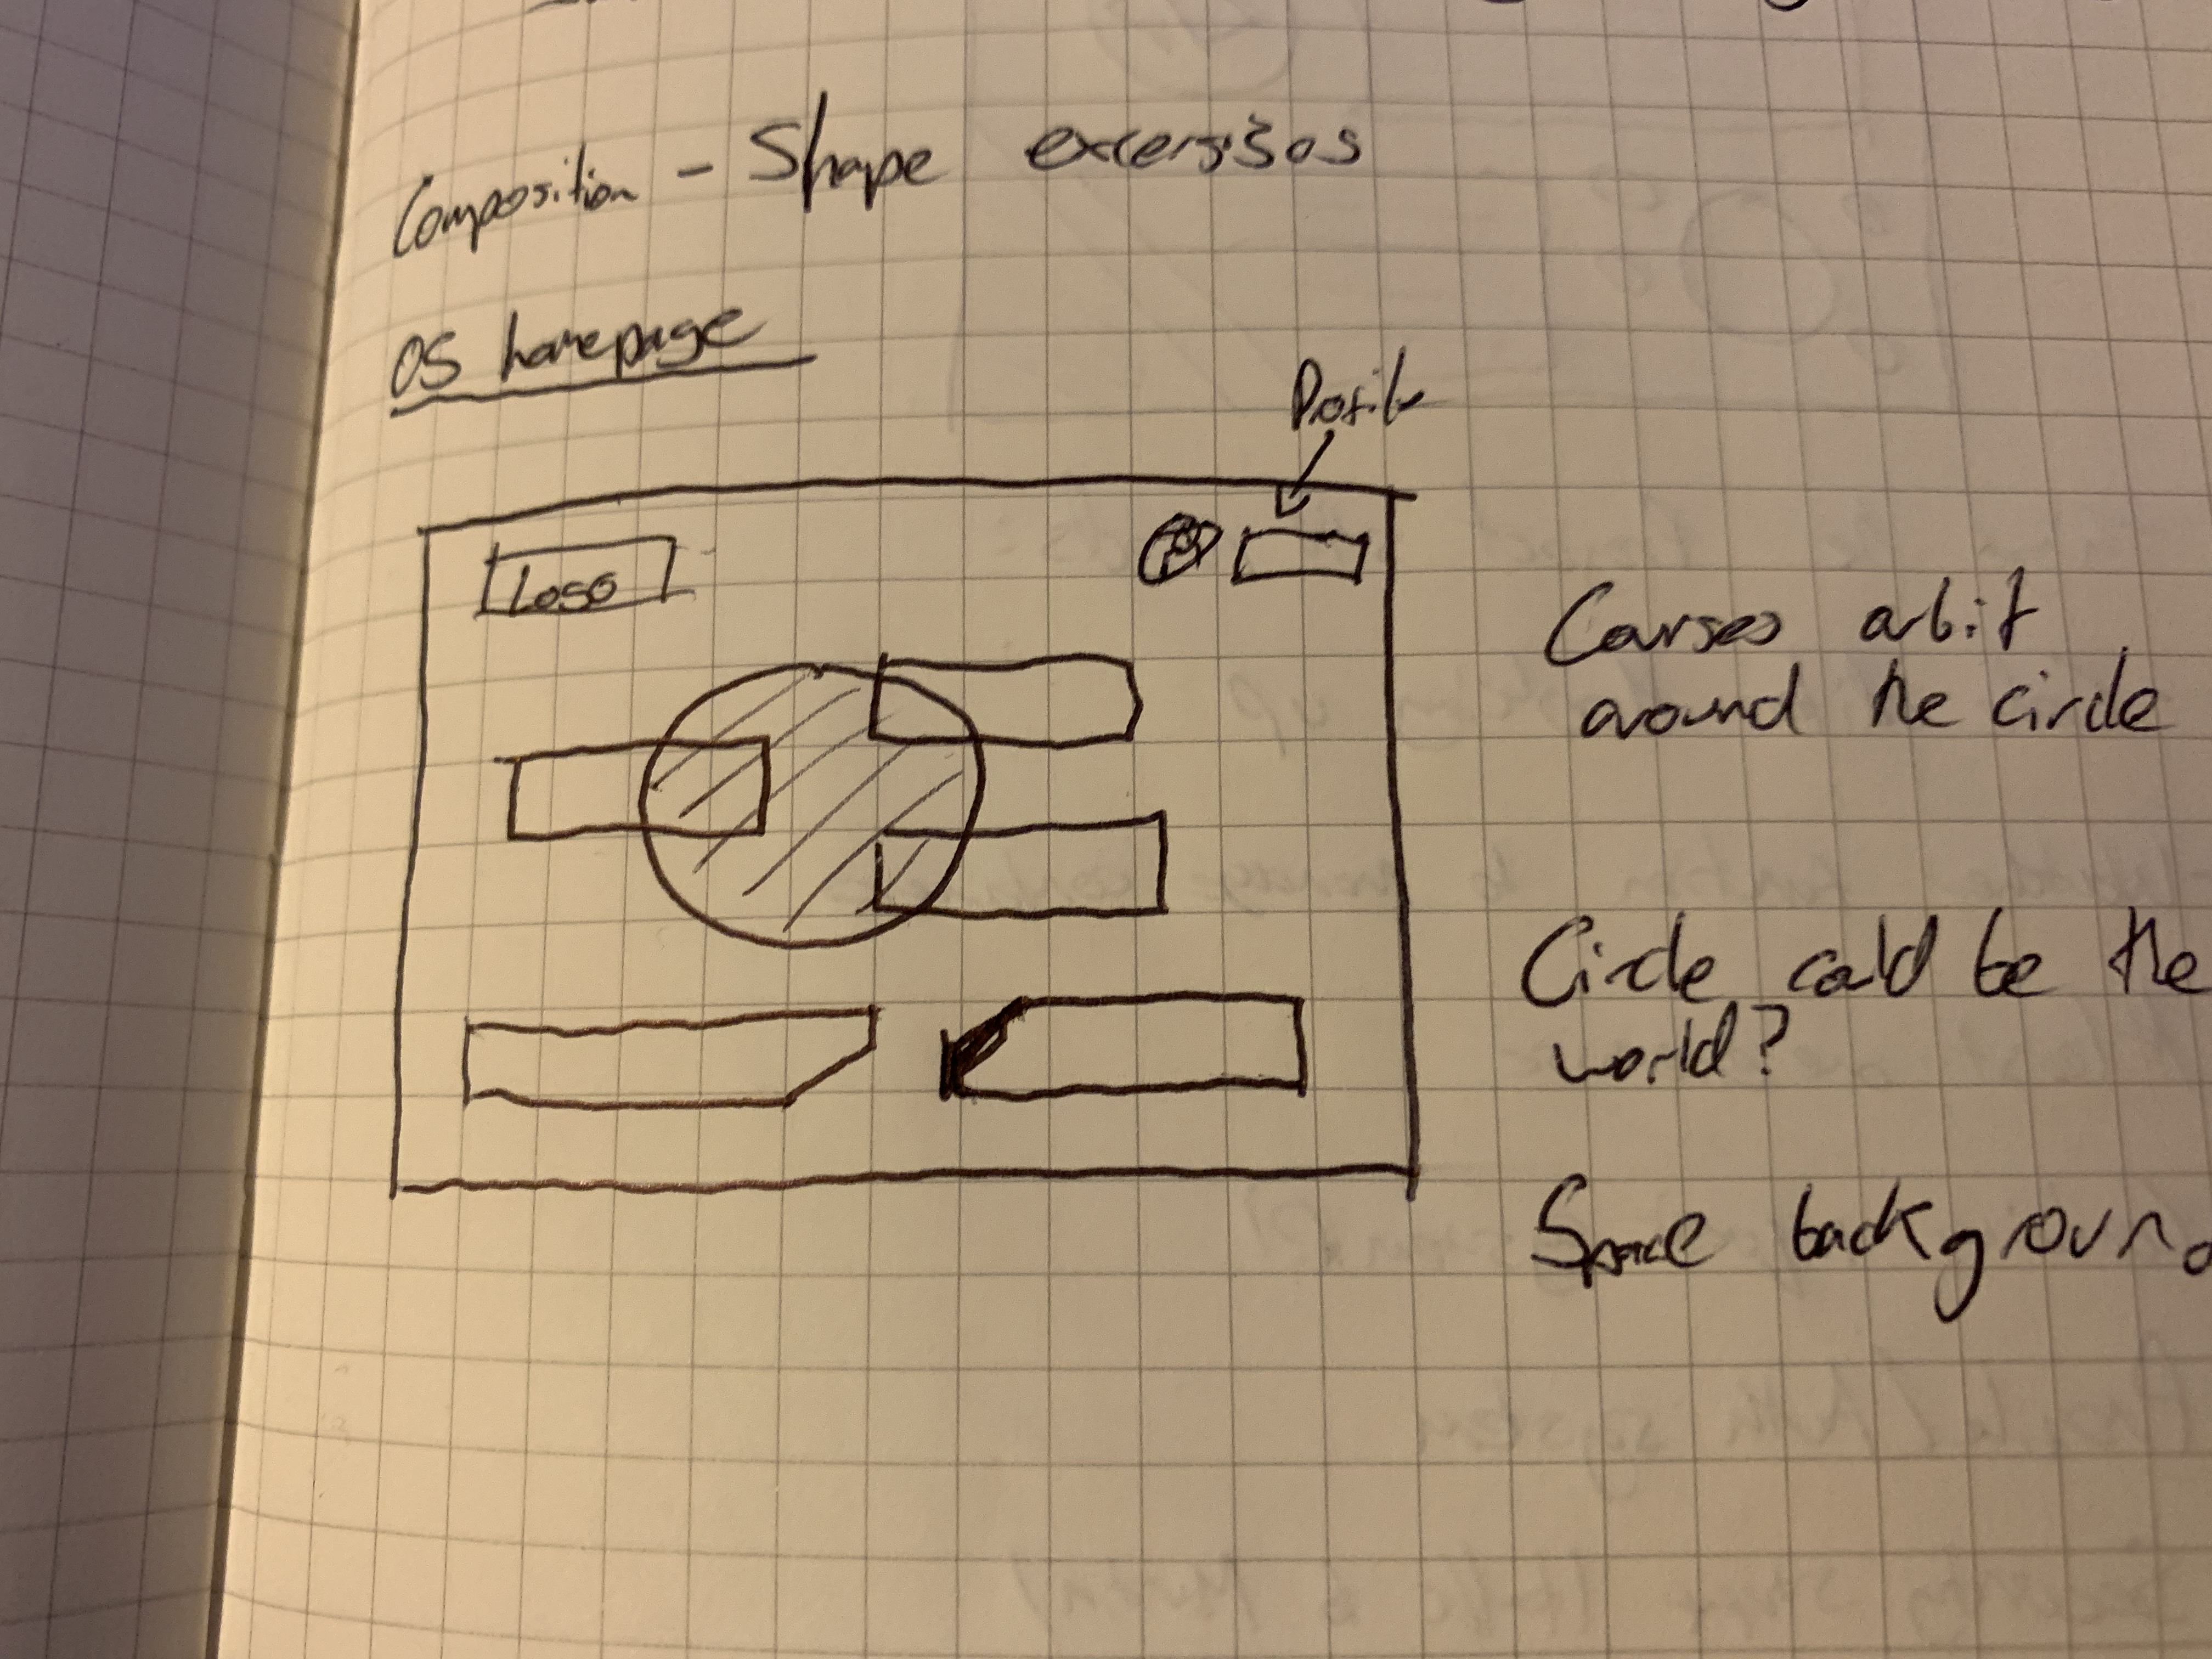
\includegraphics[width=\linewidth]{res/lofi-prototype-1.jpg}
  \caption{Prototype 1}\label{fig:lofi-prototype-1}
  \endminipage\hfill
  \minipage{0.32\textwidth}
  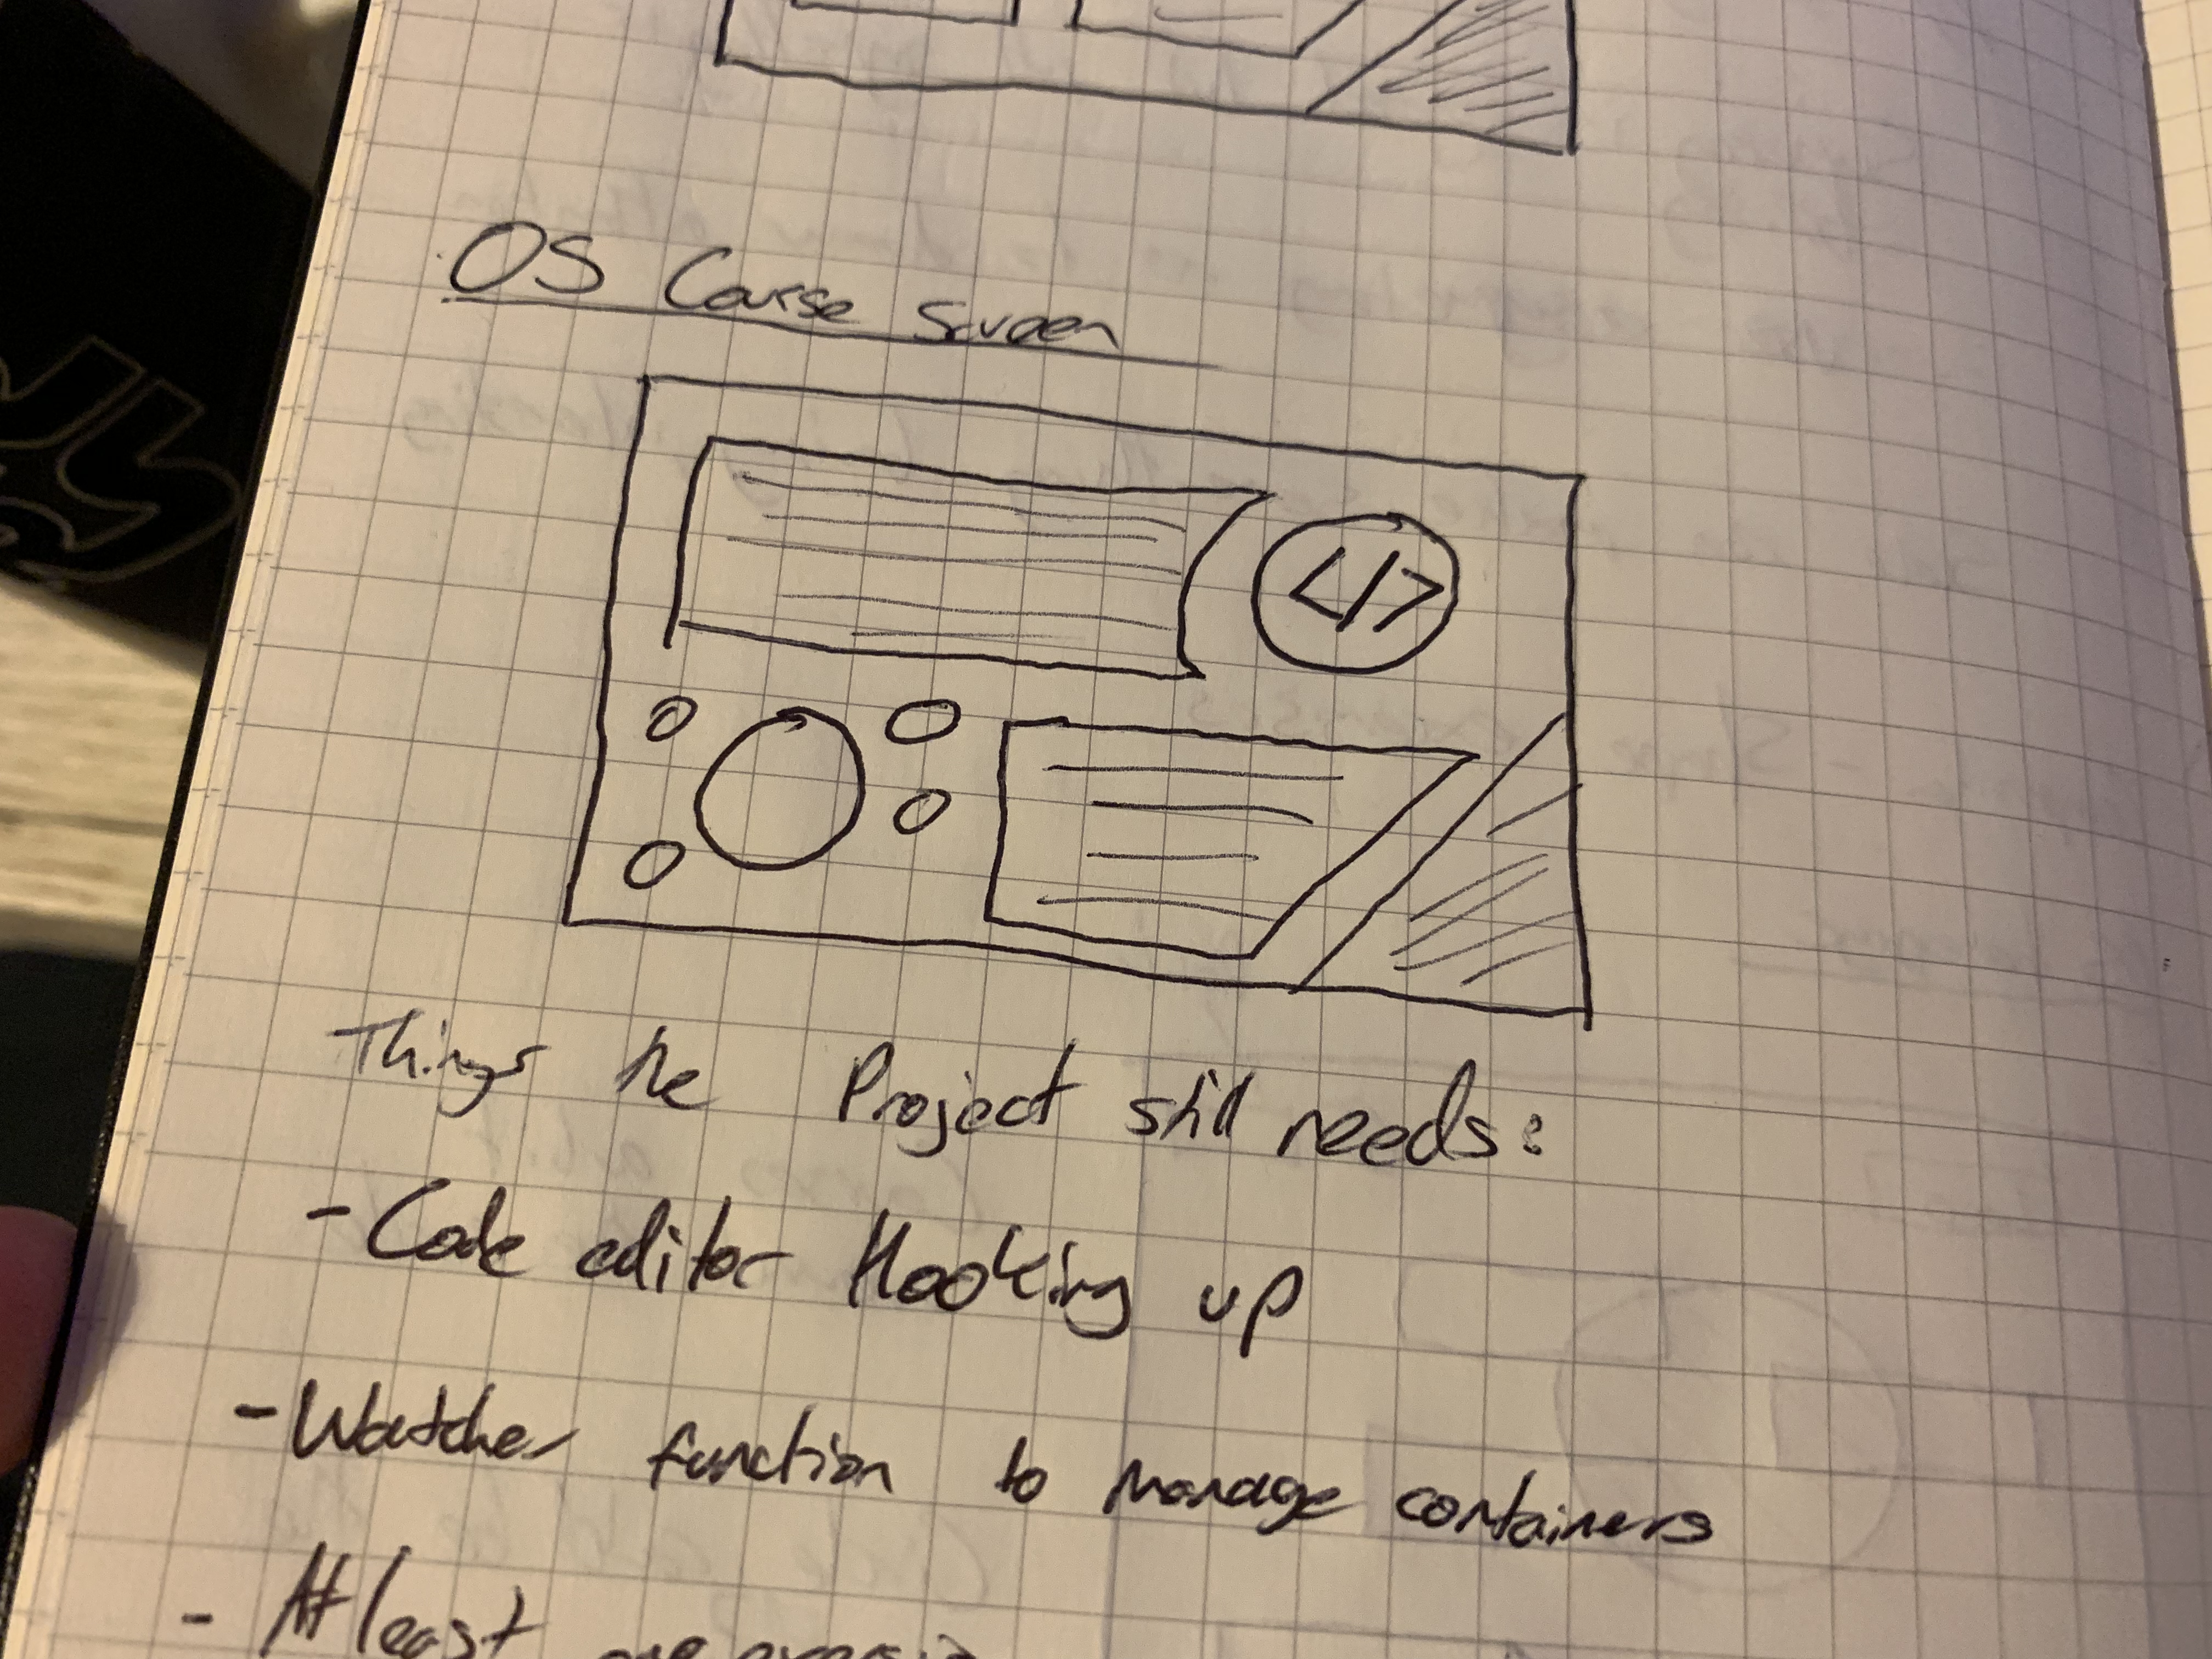
\includegraphics[width=\linewidth]{res/lofi-prototype-2.jpg}
  \caption{Prototype 2}\label{fig:lofi-prototype-2}
  \endminipage\hfill
  \minipage{0.32\textwidth}
  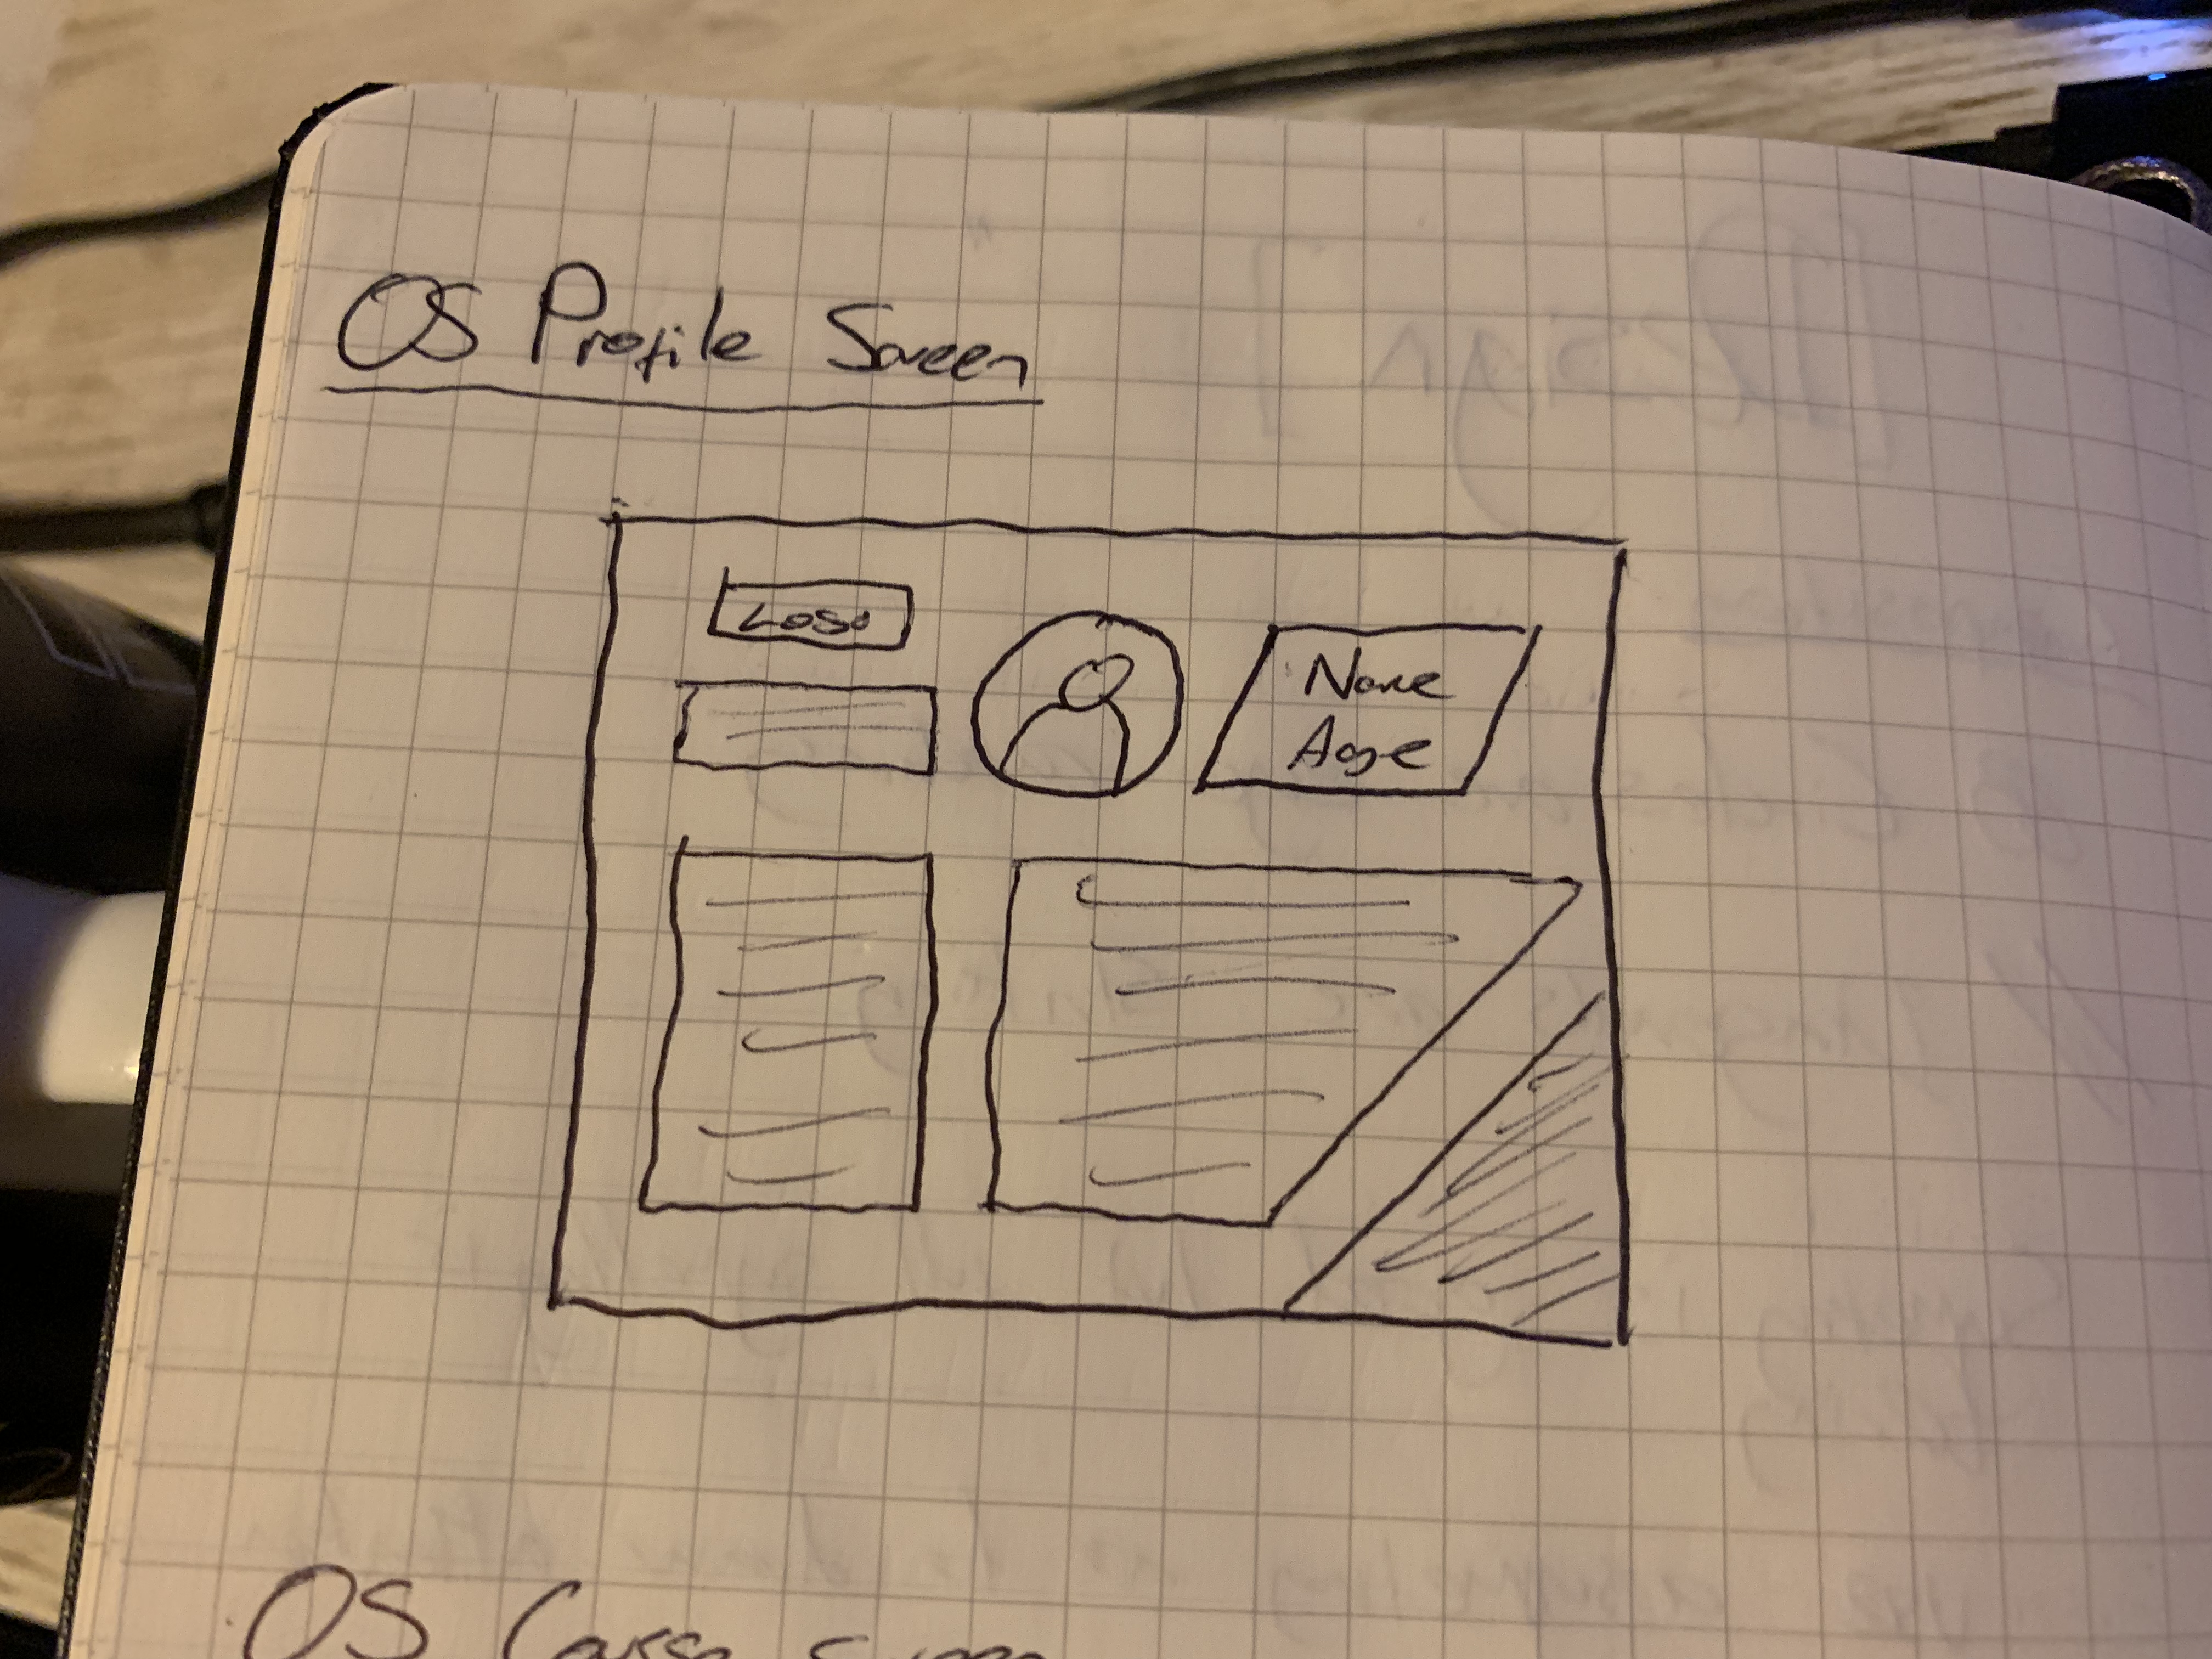
\includegraphics[width=\linewidth]{res/lofi-prototype-3.jpg}
  \caption{Prototype 3}\label{fig:lofi-prototype-3}
  \endminipage
\end{figure}

\subsection{Prototype One}

Prototype design one uses small blocks of informative text which orbit around a circular shape in the middle. Not having significantly large blocks of text means the user won't be intimidated by the information being displayed to them.

The circle is a technique that designers use in order to draw the viewers attention to a specific area. Although it is not shown in the prototype image the font styles that are in use are: one serif font for the display text (the titles and headings) and one sans serif font for the body text (bulk of text).

Some navigation elements can be seen along the top representing different sections of the site.

\subsection{Prototype Two}

Design two uses circles in the same way that prototype one does in order to draw users attention however it also uses interesting borders and shape cut offs to make the website stand out against most websites which stick with the default rectangular shape of most UI elements.

This prototype contains a lot of textual information and might be more relevant for a page that needs to convey a message to the reader that requires significant blocks of text. This design wouldn't be appropriate for a landing page but maybe would for a page on an exercise the user can do.

The font styles in use are a \texttt{monospaced} font for the display text and a sans serif font for body text.

\subsection{Prototype Three}

The third design is a concept for a profile screen but could be applied to a page that represents a particular language and technology. It has lots of space for informative textual content as well as some space for image assets/other resources that might convey information in a less traditional method.

It attempts to use more shapes in order to draw attention to certain areas of the page although it does give the page a slightly skewed look on the right hand side so perhaps if this design were to be implemented it may not render on the screen in a way that looks good.

No specific font styles were decided upon for this prototype.

\section{Overall declaration of solution chosen}

Based off of the research conducted in Chapter \ref{lit} and the potential woes of implementing some of the solutions proposed in this chapter. The current solution approach for creating a full implementation of the system is to have a Next.js frontend with a backend that uses Docker containers in order to implement virtual environments for users. The frontend will make use of the Monaco code editor and the Xterm terminal emulator. Communication between the containers and the frontend will be done with the WebSockets RTC method.

% TODO: put a diagram of the overall structure here (low level)

% TODO: talk about backend stuff here as well :(

\pagebreak
